\chapter{Text-Based Video Retrieval}
With the inception and steady rise of large video collections containing a diverse range of video topics comes the need for fast efficient retrieval. However, even small to medium-size collections are impossible for humans to be browsed manually, especially in a timely manner. Over the years, many sketch-based methods, operating with various visual features, were developed to ease retrieval in these collections \cite{KlausWikiView,BlazekAdam2015,KlausVBS2019_sketchsearch,LokocVBS2019_Nasnet}. Nonetheless, it is inherently difficult, especially for a non-skilled end user, to correctly reproduce a searched object by color, edge, or another sketch. Therefore, recently with advances in deep learning, an option to describe the searched object in natural language gained popularity \cite{SOMHunterVBS2020,LokocVBS2020_VIRET}. %{\color{red} Nonetheless the larger the collections less likely the searched scene is visually distinct to be exactly rememberable and reproducible by a human interacting with the collection. In these cases of zero visual example usually the only option is to describe a query in natural language  COZE ???}.
%We should note that even though an example image can be obtained for example from Google Images it can be completely dissimilar to the searched object in the collection since plethora of images can fit the same description.


Retrieval in video collections by textual queries, also called ad-hoc video search (AVS), represents a great challenge as it is necessary to semantically understand the content of queries and videos. %AVS differs from classical concept detection because in many cases interactions between objects needs to be captured, e.g.
For example, a query \textit{`a person talking behind a podium wearing a suit outdoors after sunset'} requires the system to understand that person is not on the podium and \textit{after sunset} means at night not while the sun is setting. Further, the same information needs to be extracted from the video to retrieve the scene. This example illustrates how AVS differs from classical concept-based retrieval -- rather, it is a combination of concept and action detection, relation modeling, and text understanding.

Since 2016 the ad-hoc video search task is annually held at TRECVid with a goal to model the end-user search use-case. Each year's task consists of 30 one-sentence queries for segments of video containing persons, objects, activities, locations, etc. and combinations of the former.
Until 2018 IACC.3 dataset \cite{2017trecvidawad} of approximately 4600 Internet Archive videos with 600 hours of content was used. In 2019 a larger high-resolution V3C1 dataset \cite{V3C1dataset} of 7475 Vimeo videos with 1000 hours of content was introduced and used onward.

In this chapter, the winning solutions of TRECVid Ad-hoc Video Search 2018 and 2019 are discussed, and a new system built upon work of the 2018 winner Li et al. \cite{XirongW2VVpp} is proposed achieving results on par with the state-of-the-art on TRECVid AVS competition data from years 2016 and 2018. On TRECVid AVS 2017 data, the proposed system improves state-of-art by ten percent showing promising future research direction. Further, the proposed system also outperforms Li et al. on our in-house dataset with over two hundred challenging queries.

\section{Related Work}\label{sec:chap2relatedwork}
%For years content-based retrieval dominated zero-example retrieval... (concept-based video retrieval vs. natural language query)
With the introduction and broad availability of convolutional neural networks for image classification \cite{AlexNet,vgg,Szegedy_2016_InceptionV3}, many works repurposed those networks for concept extraction. 
For example, team NII-HITACHI-UIT \cite{le2016nii}, the winner of TRECVid AVS 2016, utilizes multiple readily available networks for concept detection, scene description as well as dense captioning; therefore, the AVS task is reduced into text-based retrieval task in which similarity scores between query text and video semantic features are computed using inverted index structure and TF-IDF weighting.
These so-called concept-based retrieval systems are, however, limited to only fixed sets of concepts and cannot capture relations between the concepts as the only information available is \textit{present} or \textit{not present} with some confidence measure.

One of the early works that tries to learn directly the matching between images and text is by Wang et al. \cite{Wang2019}. It encodes images into 4096-dimensional vectors using VGG network \cite{vgg}. Sentences are encoded using Word2Vec \cite{word2vec} vectors transformed into 18000-dimensional space using Fisher Vectors. A set of weights is then trained to minimize the distance between these two representations.
Other work by Dong et al. \cite{Dong2018} encodes sentences by concatenating their Bag-of-Words representations, Word2Vec vectors, and RNN outputs. These vectors are then passed through a multi-layer perceptron that is trained together with the RNN to project them into visual feature space created by e.g. ResNet-152. Aside from the text-to-image-space model trained and tested using Flickr30K dataset~\cite{Flickr30k} (containing over 30 thousand images collected from the Flickr website with five captions each), the authors try to learn a text-to-video-space model utilizing MSVD dataset. The video features are extracted using the C3D network and averaged over time; however, better results are achieved by image-based ResNet-152 network instead of the 3D video network.

The above-mentioned approaches represent an image by a single vector that is considered as an aggregation of the important image regions. However, in the process of aggregation, some important information about individual regions can be lost. Lee et al. \cite{Lee_2018_ECCV} introduce Stacked Cross Attention (SCAN), which performs text to image matching by combining similarities between individual image regions and a weighted sum of individual word vectors. Image region vectors are extracted using Faster R-CNN \cite{FasterRCNN} pre-trained on Visual Genomes dataset \cite{krishna2017visual} and one linear trainable layer is added to project the fixed region representations. Word vectors are produced by a trainable bi-directional GRU layer.

\begin{figure}
    \centering
    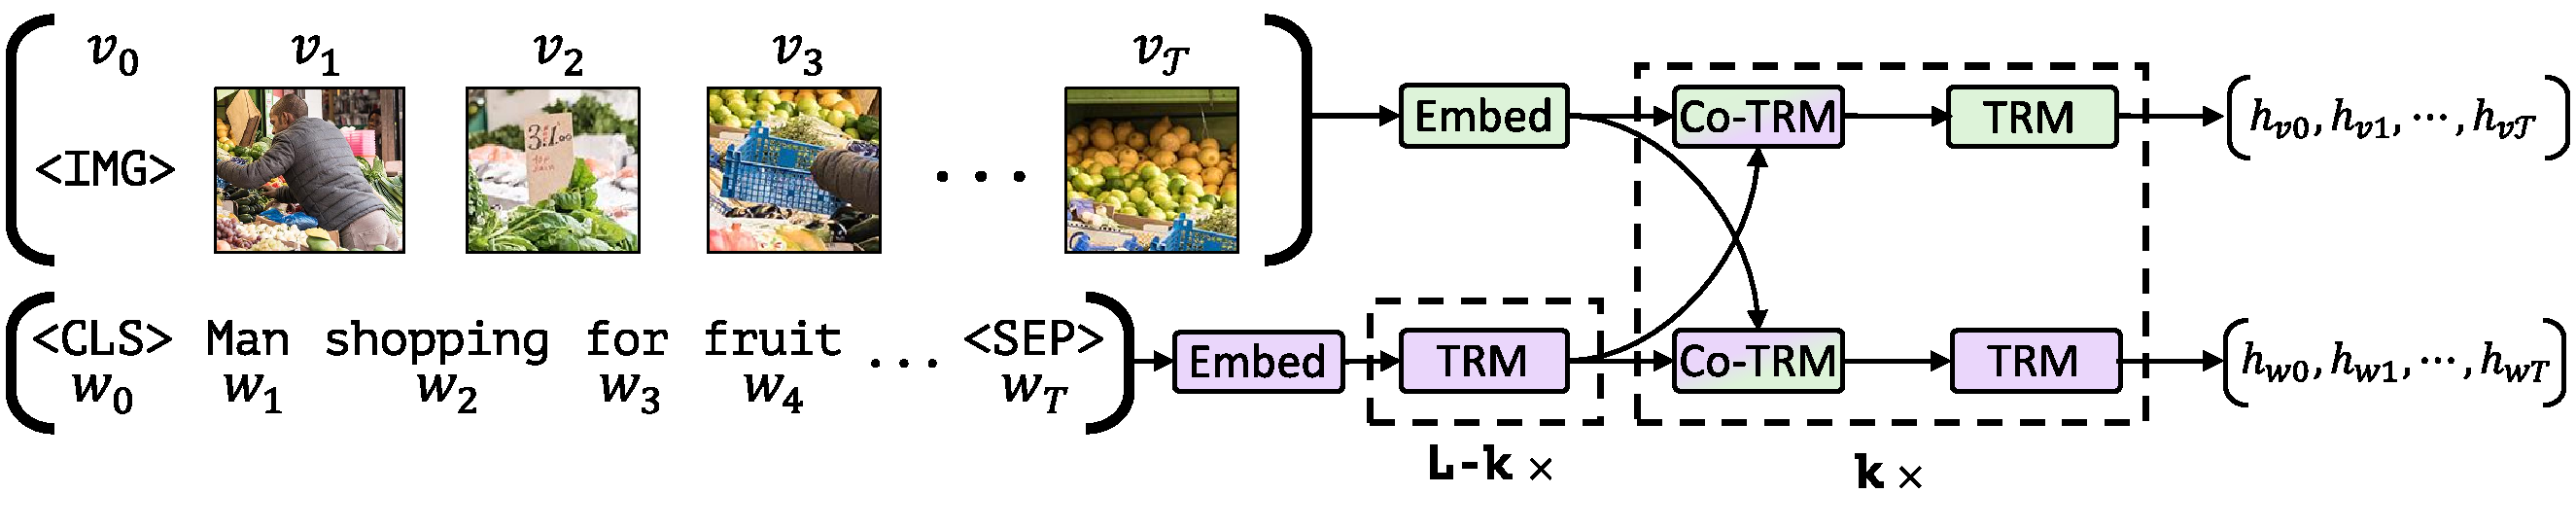
\includegraphics[width=0.95\textwidth]{img/vlbert_converted.pdf}
    \caption[ViLBERT model for image/description matching]{ViLBERT model \cite{ViLBERT} operates over image regions and text segments. Each stream is a series of transformer and co-attentional transformer layers enabling information exchange between modalities.}
    \label{fig:vlbert}
\end{figure}
ViLBERT \cite{ViLBERT} network by Lu et al. (shown in Figure \ref{fig:vlbert}) takes attention-based approach a step further by repurposing BERT attention-based bidirectional language model \cite{bert}. The original BERT processes each word (token) of an input sentence independently -- the only context is obtained through dozens of attention layers. With pretraining on a large language corpus, BERT and its variants achieved state-of-the-art results in many natural language processing tasks via transfer learning. ViLBERT's input consists of image description and set of image region features that are extracted the same way as in the work Lee et al. The network is pre-trained on large Conceptual Captions \cite{sharma2018conceptual} dataset to predict alignment score i.e. whether an image description matches a set of image regions' features. In the end, the network is finetuned on a manually annotated high-quality Flickr30K dataset. The finetuning is performed by computing the alignment score for the correct image-text pair and other three sampled incorrect pairs. The scores are passed through softmax, and cross-entropy loss is computed. The twelve attention layers in ViLBERT outperform SCAN with only one attention in image retrieval on the Flickr30K dataset by almost 20\% in terms of Recall@1 (recall at the first position) and by over 7\% in Recall@10.

As mentioned by Dong et al., simply exchanging 2D features from networks such as ResNet for 3D features extracted by e.g. C3D is not sufficient to perform video retrieval. Moreover, they imply that video retrieval can be performed with better results by extracting only 2D features. However, it is unfortunate that, by operating only on single frames, some information about actions, etc. is inevitably lost. Work of Mithun et al. \cite{Mithun2018} argues that 3D video features such as I3D and 2D image features produced by e.g. ResNet focus on different characteristics and are complementary in some sense. The first focuses on action identification and the later on identifying objects in the frames. Therefore the authors introduce two spaces: activity-text space and object-text space. A text query is then evaluated in both spaces independently, and the fusion of those two rankings is performed. Nonetheless, work of Yu et al. \cite{Yu_2018_ECCV} utilizing again only image-based ResNet-152 for feature extraction outperforms Mithun et al. by 45\% for both Recall@1 and Recall@10 in video retrieval task on MSR-VTT \cite{Xu_2016_CVPR} dataset (containing 10 thousand web video videos with 200 thousand short clips each paired with text descriptions).

\subsection{Weakly Supervised Approaches}
\begin{figure}
    \centering
    \begin{equation}\label{eg:maxmarginrankingloss}
        \begin{split}
        \min\sum_{i=1}^{|\mathcal{B}|} \left( \sum_{j\in \mathcal{N}(i)}\right. [\delta & + S(V_i,C_j) - S(V_i,C_i)]_+ \\
        & \left. + \sum_{j\in \mathcal{N}(i)} [\delta + S(V_j,C_i) - S(V_i,C_i)]_+ \right)
        \end{split}
        % \min\sum_{j\in \mathcal{N}(i)}\left(\left[\delta + S(V_i,C_j) - S(V_i,C_i)\right]_+ + \left[\delta + S(V_j,C_i) - S(V_i,C_i)\right]_+\right)
    \end{equation}
    \begin{equation}
        \max\ \sum_{i=1}^{|\mathcal{B}|} \log \left(\frac{e^{S(V_i, C_i)}}{e^{S(V_i, C_i)}+\sum_{j \in \mathcal{N}(i)} \left[e^{S(V_i, C_j)} + e^{S(V_j, C_i)}\right]}\right)\label{eg:nceloss}
    \end{equation}
    
    \caption[Max-margin ranking loss and noise-contrastive estimation loss.]{Max-margin ranking loss and noise-contrastive estimation loss. $S(V_i,C_j)$ is a similarity score between video clip $V_i$ and caption $C_j$, $\mathcal{N}(i)$ is a set of negatives for video/caption $i$, $\delta$ is the margin and $\left[\cdot\right]_+$ is $max(0, \cdot)$. In \cite{Miech_2020_CVPR} authors allow for multiple positive pairs $\mathcal{P}(i)$ due to uncertainty in video-caption alignment by substituting $e^{S(V_i, C_i)}$ for $\sum_{(x,y)\in\mathcal{P}(i)}e^{S(V_x, C_y)}$.}
\end{figure}

Learning mappings of text and videos into joint embedding space often requires large manually annotated datasets. Even though there are datasets such as MSR-VTT or Tumblr GIF (TGIF) \cite{Li_2016_CVPR}, each with more than 100 thousand short clips (or gifs in the latter case) with their natural language descriptions, the work of Miech et al. \cite{Miech_2019_ICCV_HowTo100M} shows that even much larger datasets are greatly beneficial to video retrieval. The authors introduce HowTo100M dataset containing 136 million video clips from 1.22 million narrated instructional web videos, each accompanied by automatically or human-generated audio transcriptions. Although the transcriptions need not to align with the visual content or they may be unrelated completely, a simple shallow network trained max-margin ranking loss (Equation \ref{eg:maxmarginrankingloss}) achieves state-of-the-art results on multiple benchmarks.
For video, the network utilizes 2D and 3D features extracted by Resnet-152 pre-trained on ImageNet and ResNeXt-101 pre-trained on Kinetics respectively. The features are then aggregated by temporal max-pooling and concatenated. Transcriptions are embedded using Word2Vec and a shallow 1D convolutional network is used to extract fixed-sized representation. Further, a single linear fully-connected layer with a two-layer context gating function is used for both the visual and textual features. The authors stress that, during training, intra-video negative sampling strategy is critical for good performance -- half of the negative pairs in the loss belong to the same original video to ensure that the learned embedding focuses on relevant aspects of the video clip.

In video retrieval task on the MSR-VTT dataset, this network achieves very similar results as Mithun et al.; however, the network is only trained on HowTo\-100M. Finetuning on MSR-VTT improves the results of Mithun et al. by more than 110\% in Recall@1 and 77\% in Recall@10. Additional work by the authors \cite{Miech_2020_CVPR} shows the benefits of training video feature extractors (I3D or S3D) from scratch. Further it is suggested that noise-contrastive estimation loss (\cite{ExploringLimitsLanguageModeling}, Equation \ref{eg:nceloss}) outperforms standard max-margin ranking loss.


\subsection{Winners of TRECVid Ad-hoc Video Search}\label{sec:winnersOfTrecvid}
This section summarizes approaches used by winning teams of TRECVid AVS challenge. Namely, it focuses on Dual Encoding by Dong et al. \cite{Dong_2019_CVPR} and Word-To-Visual-Vector (W2VV++) by Li et al. \cite{XirongW2VVpp} (shown in Figure \ref{fig:w2vvpp_original_sketch}) since these have been used in the winning submissions of 2018 and 2019 \cite{wu2019hybrid, li2018renmin, li2019renmin}.


\begin{figure}
    \centering
    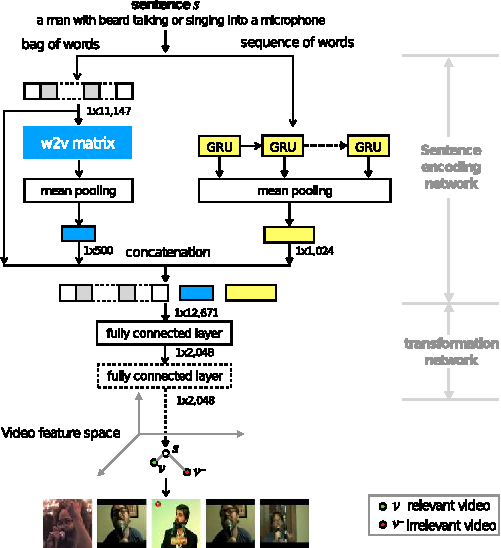
\includegraphics[width=0.6\textwidth]{img/w2vvpp_converted.pdf}
    \caption[A diagram of W2VV++ model]{A diagram of the original version of W2VV++ model, taken from \cite{XirongW2VVpp}.}
    \label{fig:w2vvpp_original_sketch}
\end{figure}

\begin{description}[labelwidth=1em, leftmargin=!]
    \item \textbf{Frame features.} Image-based 2D CNNs are used to extract features for individual frames. In particular Li et al. utilizes two CNNs: ResNeXt-101 from \cite{ImageNetShuffle} and ResNet-152 from MXNet library \cite{mxnet} %\cite{DL-61-86 at TRECVID 2017: Video-to-Text Description}
    both trained on the ImageNet dataset with over 10 million images and over 10 thousand classes.
    Frames are resized to $256\times 256$ and CNN features (the output of the penultimate layer) are extracted from its 10 sub-images (i.e. five $224\times 224$ center and corner patches, all of them also horizontally flipped). The final frame features are the result of averaging those ten sub-image features and concatenation of ResNeXt-101 and ResNet-152 features.

    \item \textbf{Video features.} For a given video clip frames are sampled every 0.5 seconds. Features for each frame are extracted as described above. Then the features are aggregated by one or more of the following approaches: (1) averaging features over time. (2) using a bidirectional recurrent neural network with e.g. GRU units with outputs of both directions concatenated and averaged over time. (3) using 1D convolution with outputs averaged over time. (4) computing differentiable version of VLAD (Vector of Locally Aggregated Descriptors) -- NetVLAD \cite{Arandjelovic_2016_CVPR}. (5) using graph network \cite{Mao_2018_ECCV_Workshops} to learn a fixed-sized hierarchical representation of the video among frames.
    
    Wu et al. \cite{wu2019hybrid} utilize averaging over time (1). Further GRU (2), NetVLAD (4), graph network (5) are run in parallel on top of frame features.
    Video representation of Dong et al. \cite{Dong_2019_CVPR} concatenates output of the approach (1), GRU (2) and 1D CNN (3) run on top of the GRU features. Li et al. \cite{XirongW2VVpp} use only the feature averaging over time.
    
    \item \textbf{Word features.} Over the years multiple approaches to word embeddings have been developed. All three mentioned works adopt a pre-trained 500-dimensional Word2Vec model trained on English tags associated with 30 million Flickr images supporting over 1.7 million words \cite{Dong2018}. The 2019 version \cite{li2019renmin} of W2VV++ system by Li et al. also takes advantage of pre-trained BERT \cite{bert} sub-word embeddings.
    
    \item \textbf{Sentence features.} One of the simplest representation is bag-of-words (BoW). The work of Li et al. constructs BoW by taking all words from a training set, excluding those that occur less than five times and those contained in the NLTK stopword list. Aside from the BoW features, Li et al. utilize Word2Vec pre-trained embeddings and single layer 1024-dimensional GRU network. The outputs of both methods are averaged over all words and concatenated together with BoW into $(500+1024+11147)$-dimensional vector. %The 2019 version also adds 1024-dimensional pre-trained BERT embeddings also averaged over all input tokens.
    Works of Wu et al. and Dong et al. embed words using the Word2Vec pre-trained embeddings and use the same architecture as they use for video feature extraction. Further, they also allow to fine-tune the embeddings.
    
    \item \textbf{Loss function.} Li et al. and Dong et al. project sentence features and video features into the common vector spaces by a single fully-connected layer followed by hyperbolic tangent or batch normalization respectively. Then all the approaches adopt max-margin ranking loss (Equation \ref{eg:maxmarginrankingloss}) with hard negatives \cite{VSEpp}, i.e. $\mathcal{N}(i)=\textrm{argmax}_{j\neq i} S(V_i, C_j)$ or $\textrm{argmax}_{j\neq i} S(V_j, C_i)$ for the first and the second term respectively. The idea behind the hardest negative can be intuitively explained by the fact that the hardest negative determines success or failure in the Recall@1 metric. For practical reasons, the hardest negative is selected only from mini-batch instead of the whole dataset. The work of Li et al. further only uses the second term in the max-margin ranking loss with negatives for videos but not for sentences.
    % \item \textbf{Train, validation and test sets.}
\end{description}



\clearpage
\section{Our Method}\label{sec:chap2ourmethod}
As already mentioned, text-to-visual matching systems usually employ pre-\linebreak[4]trained visual and text feature extractors and learn only the mapping between these features. While some work focuses on training video feature extractors \cite{Miech_2020_CVPR}, to the best of our knowledge, no work trains advanced text feature extractors. The authors of \cite{Miech_2020_CVPR} prove that training the whole video extractor benefits from the performance if large, even only automatically annotated, datasets are available. In this work, we experimentally prove the same for the text extractor. For that we adopt Transformer-based \cite{AttentionisAllyouNeed} state-of-the-art model RoBERTa \cite{RoBERTa}, pre-trained on large corpora of English texts from the internet such as Wikipedia and news articles. Even though Transformers have already been used in the text-to-visual systems, e.g. Renmin University at TRECVid 2019 \cite{li2019renmin} and Contrastive Bidirectional Transformer \cite{ContrastiveBidirectionalTransformer} both utilized pre-trained BERT or Miech et al. \cite{Miech_2020_CVPR} adopted one Transformer's attention layer into their language part of the system; we show that training the whole Transformer network for this task is beneficial.

\subsection{Problem Statement} Given a video $V=\{v_1, \ldots, v_n\}$ with frames $v_i$ and a text caption $C=\{c_1,\ldots,c_m\}$ with words $c_i$, we aim to learn a mapping of the video $f(V; \theta_f)$ into $\R^d$ and a mapping of the caption $g(C; \theta_g)$ to the same space $\R^d$ such that similarity $S(V, C)$ is maximized for a video-caption pair, if the caption describes correctly the video, and minimized for a pair, if the caption does not describe the video. Note, we will omit the parameters $\theta_f$ or $\theta_g$ and refer to both the functions and their parameters by only $f$ or $g$ for simplicity. We define the similarity as cosine of $f(V)$ and $g(C)$ as
\begin{equation}
    S(V, C)=\frac{f(V)^\top g(C)}{\|f(V)\|_2\|g(C)\|_2}.
\end{equation}

In this framework, text retrieval in a video database $\mathcal{DB}$ is solved by computing $f(V_i)$ for all videos $V_i$. Given a query $Q$, $g(Q)$ is computed and for each video similarity scores $S(V_i, Q)$ are computed and the videos with the highest scores are returned. Since $f(V_i)$ can be precomputed and $g(Q)$ can be considered as a constant for a query of limited length, the time complexity is determined by the size of the database and the dimension $d$ of the joint space $\R^d$, i.e. $O(|\mathcal{DB}|d)$. Note, in practice, a video can contain many unrelated segments while the query usually describes only one segment; therefore, videos are split into individual shots, i.e. in the context of this thesis $V_i$ is not the whole video but only a single shot.


\subsection{Video Representation}
For video representation we use the W2VV++ (Word-To-Visual-Vector) system~\cite{XirongW2VVpp} developed by Li et al. As described in Section \ref{sec:winnersOfTrecvid} a frame is extracted every 0.5 seconds, it is resized into $256\times 256$ and features are extracted from its 10 sub-images. The features are obtained by ResNext-101 \cite{ImageNetShuffle} and Resnet-152 \cite{mxnet} both trained on ImageNet. The features are averaged across the image patches and all the video frames resulting in a fixed 4096-dimensional vector.

The only trainable part of the video mapping function $f$ is a single fully-connected layer with hyperbolic tangent, i.e. the whole video mapping function is as follows:
\begin{equation}
    f(V)=\tanh\left(W_f\mathcal{N}(V)+b_f\right)
\end{equation}
where $\mathcal{N}(\cdot)$ is the non-trainable mapping to 4096-dimensional space by CNNs averaged over frames described in the previous paragraph, $W_f\in\R^{d\times 4096}$ and $b_f\in \R^d$ are the trainable weights and biases.

\subsection{Text Representation}
Similarly to Li et al. three components are utilized -- Bag of Words, Word2Vec, and newly BERT instead of RNN. Specifically, the Bag of Words component is defined as
\begin{equation}
    BoW(C)=\left(\#(w_1, C),\ldots,\#(w_{|\mathcal{V}|}, C)\right)
\end{equation}
where $w_i\in\mathcal{V}$ are words from a vocabulary and $\#(w,C)$ is number of occurrences of a word $w$ in the text $C$. We use the same vocabulary as Li et al. with $|\mathcal{V}|=11147$ words.

Word2Vec component utilizes a pre-trained 500-dimensional model trained on English tags associated with 30 million Flickr images supporting over 1.7 million words \cite{Dong2018}. A text caption $C$ is represented by the average of the individual word embeddings $e(c_i)$. The embedding is not fine-tuned and stays fixed throughout the whole training.
\begin{equation}
    W2V(C)=\frac{1}{|C|}\sum_{i=1}^{|C|}e(c_i)
\end{equation}

The last component of the text architecture is BERT neural network \cite{bert}. BERT's architecture is a multi-layer bidirectional Transformer encoder based on the work by Vaswani et al. \cite{AttentionisAllyouNeed} (Figure \ref{fig:original_bert}). It uses only self-attention and point-wise, fully connected layers stacked into transformer blocks with information passing between words (sub-words) only via the self-attention. In our work, we use the 110 million parameter variant of BERT called $\mathrm{BERT_{BASE}}$ with 12 Transformer blocks, size of the hidden layers 768, and 12 self-attention heads. For detailed architecture description, we point readers to the original work of Vaswani et al.~\cite{AttentionisAllyouNeed} and the BERT paper \cite{bert}.

BERT outputs a 768-dimensional vector for each input sub-word. We average all sub-word vectors to obtain representation $BERT(C)$ of the original text caption $C$.
We initialize BERT's weights by the ones provided by the authors of \textit{RoBERTa: A Robustly Optimized BERT Pretraining Approach} \cite{RoBERTa} and further train them on our dataset.

Similarly to the video network, the text network $g$ ends by concatenating the text representations and applying a fully-connected layer with hyperbolic tangent and projects a text caption into the joint text-video space:
\begin{equation}
    g(C)=\tanh\left(W_g\left[BoW(C); W2V(C); BERT(C)\right]+b_g\right).
\end{equation}
In the equation, $\left[\ldots\right]$ is vector concatenation, $W_g\in\R^{d\times (11147+500+768)}$ and $b_f\in \R^d$ together with all the weights of BERT are the trainable parameters of $g$.

\begin{figure}
    \centering
    \newcolumntype{C}[1]{>{\centering\arraybackslash}p{#1}}
    \begin{tabular}{cC{0.7cm}cC{0.7cm}c}
    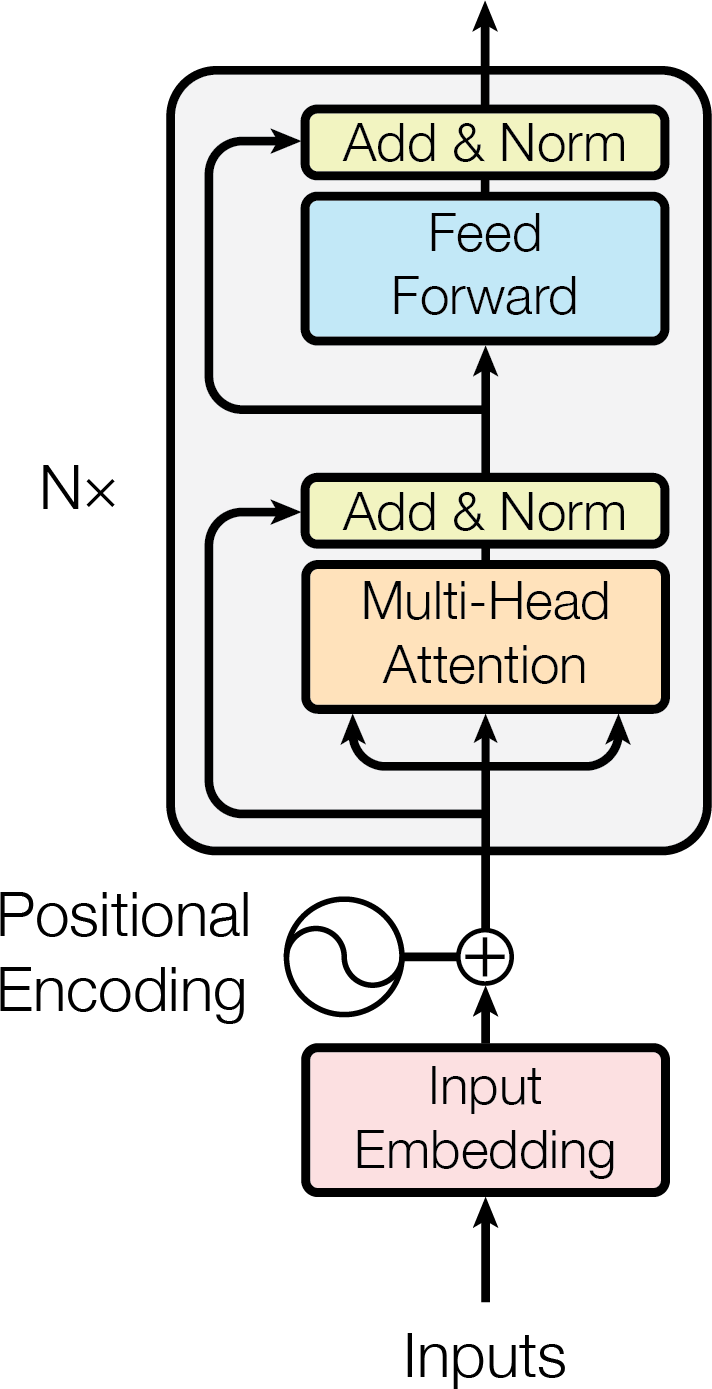
\includegraphics[align=c,width=.2\textwidth]{img/bert/bert.png}
    &
    &
    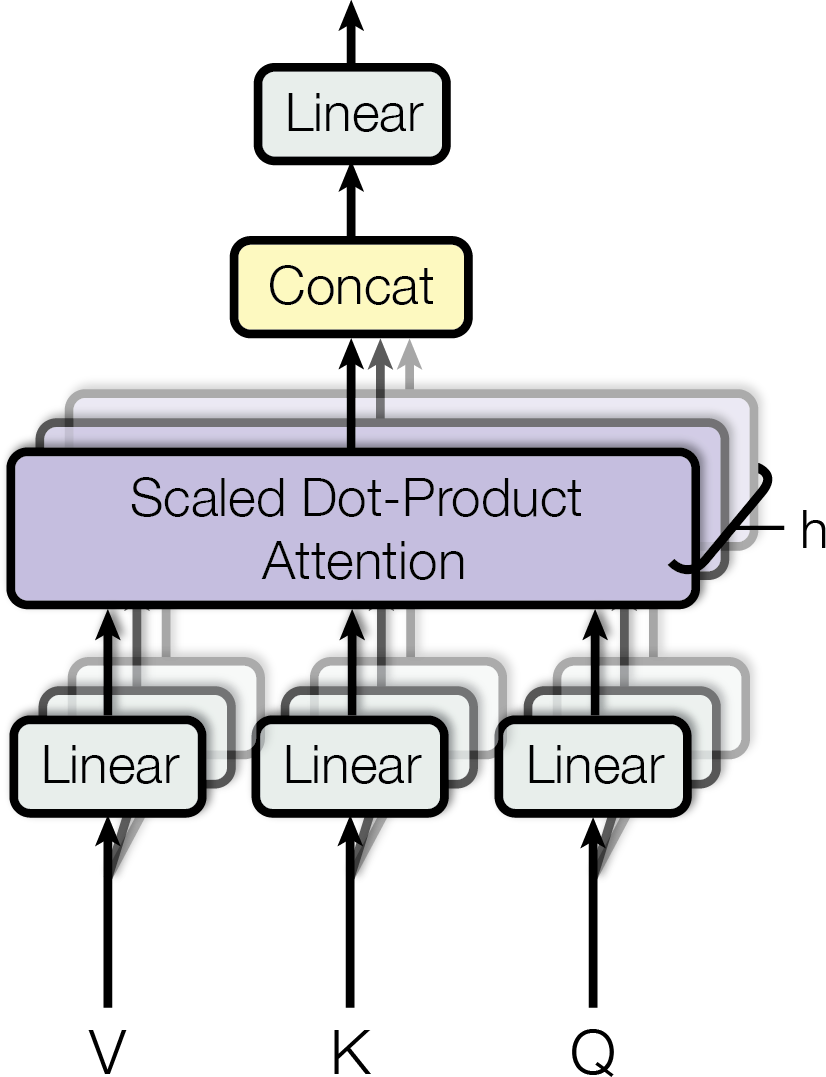
\includegraphics[align=c,width=.25\textwidth]{img/bert/bert-attention.png}
    &
    &
    
    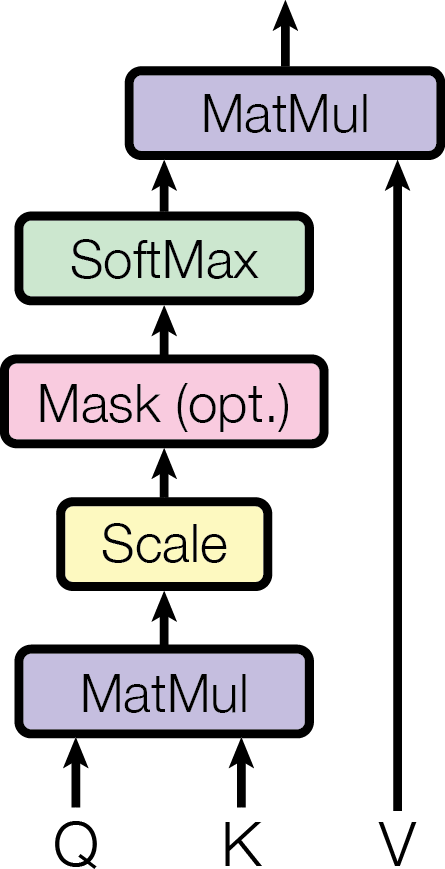
\includegraphics[align=c,width=.15\textwidth]{img/bert/bert-singleattention.png}
    \end{tabular}
    \caption[Schema of Transformer-based encoder such as BERT]{Schema of Transformer-based encoder such as BERT (left), multi-head attention (middle), and single scaled dot-product attention (right). Images from \cite{AttentionisAllyouNeed}.}
    \label{fig:original_bert}
\end{figure}

\subsection{Loss Function}
Our work employs the same variant of max-margin ranking loss (Equation \ref{eg:maxmarginrankingloss}) as Li et al. Specifically, the term with caption negatives is ignored and the set of video negatives contains only the hardest negative from a batch $\mathcal{B}$:
\begin{equation}\label{eq:our_loss}
    \min\sum_{i=1}^{|\mathcal{B}|}\left[\delta + \textrm{argmax}_{j\neq i} S(V_j, C_i) - S(V_i,C_i)\right]_+.
\end{equation}
We discuss the decision and compare other losses in the next section.



\clearpage
\section{Experiments}\label{sec:chap2experiments}
We first describe datasets used in our experiments for training, validation, and testing together with metrics used for evaluation. Then in Section \ref{sec:trainingDetails} training details are provided. Section \ref{sec:chap2results} presents the results of our model and compares them to the related work, mainly W2VV++ \cite{XirongW2VVpp}. Finally, an ablation study in Section \ref{sec:chap2ablation} justifies key design choices such as the loss function.

\subsection{Datasets and Evaluation Metrics}
We use the same train, validation and test sets as in the work of Li et al. with the features provided by the authors\footnote{\label{note:1}Publicly available at \url{https://github.com/li-xirong/avs}.}. For train set MSR-VTT \cite{Xu_2016_CVPR} and Tumblr GIF (TGIF) \cite{Li_2016_CVPR} is used. TGIF dataset contains over 100 thousand animated GIFs with their natural language captions. MSR-VTT dataset contains 200 thousand short clips each paired with text descriptions in 10 thousand videos.
For validation is used TRECVID 2016 Video-to-Text task dataset \cite{awad2016trecvid} with two thousand Vine videos each described by a sentence by two annotators. To stay consistent with Li et al. we utilize only 200 videos provided by the authors\footref{note:1}.
Testing is performed on the IACC.3 dataset \cite{2017trecvidawad} used for TRECVid AVS task from 2016 to 2018 containing approximately 4600 Internet Archive videos with 600 hours of content. The videos are split into 335,944 short clips by automatically detected shot boundaries provided by the authors of the dataset.
Further for testing we use over two hundred sentence-based queries manually collected for 20 thousand frames uniformly sampled from the V3C1 dataset (dubbed 20k-V3C1).

Suppose we have a set $\mathcal{Q}=\{\left(C_i,\mathcal{T}_i\right)\}_i$ of caption-video pairs with the possibility that a caption $C_i$ can correspond to many target videos $V\in\mathcal{T}_i$. Given a query (text caption) $C$ a model asigns each video $V$ a position (rank) in the result list $r(C, V)$. Good model will assign low $r(\cdot, \cdot)\to 1$ for relevant videos and large $r(\cdot, \cdot)\to |\mathcal{DB}|$ for irrelevant ones. We use the following metrics to measure model performance. Recall@k (R@k) is defined as:
\begin{equation}
    \mathrm{Recall@k}=\frac{1}{|\mathcal{Q}|}\sum_{\left(C_i,\mathcal{T}_i\right)\in \mathcal{Q}}\left(\frac{1}{|\mathcal{T}_i|}\sum_{V\in \mathcal{T}_i} [\![r(C_i,V)\leq k]\!]\right)
\end{equation}
where $[\![\cdot]\!]$ is indicator function which is one if the argument is true and zero otherwise. As we use Recall@k in scenario where there is always only a single target video ($\mathcal{T}_i=\{V_i\}$) the expression in the bracket can be simplified into $[\![r(C_i,V_i)\leq k]\!]$.
Further, the official TRECVid AVS metric is based on mean average precision (mAP). The standard mAP is defined as:
\begin{equation}
    \mathrm{mAP}=\frac{1}{|\mathcal{Q}|}\sum_{\left(C_i,\mathcal{T}_i\right)\in \mathcal{Q}}\left(\frac{1}{|\mathcal{T}_i|}\sum_{V\in \mathcal{T}_i}
    \frac{\left|\{\nu\in\mathcal{T}_i\ |\ r(C_i,\nu)\leq r(C_i,V)\}\right|}{r(C_i,V)}\right)
\end{equation}
where the innermost fraction is Precision@k with $k=r(C_i,V)$. If the set of target videos $\mathcal{T}_i$ contains only one video $V_i$ the metric is also called mean reciprocal rank (MRR) $1/|\mathcal{Q}|\cdot\sum_{\left(C_i,\{V_i\}\right)\in \mathcal{Q}}1/r(C_i,V_i)$.


Since it is difficult to evaluate all 335,944 shots from IACC.3 manually, performance at TRECVid AVS task is measured by inferred average precision (infAP) \cite{infAP}. Compared to standard (mean) average precision it eliminates bias created by only manually labeling the retrieved shots while unretrieved shots are not labeled.

\subsection{Training Details}\label{sec:trainingDetails}
In all our experiments, unless otherwise stated, the joint space dimension $d$ is set to $2048$.
Prior training, weights $W_f$ and $W_g$ are initialized by Glorot initiali\-zer~\cite{Xavier_Glorot_init}, biases $b_f$ and $b_g$ are initialized by zeros and BERT network by pre-trained weights from \cite{RoBERTa}. Batch size of 96 clip-text pairs is selected to fit into 16GB of VRAM of a Tesla V100 GPU. We use the Adam optimizer \cite{Adam14} with a learning rate of $10^{-5}$ and linear warm-up for the half of the first epoch (approx. 1700 steps). The learning rate is linearly decayed to zero in a span of 60 epochs; however, the best performing model on the validation set is selected which is usually achieved after approximately ten epochs. With the video features extracted beforehand, the training itself takes a few hours on a single Tesla V100 GPU. Pytorch and its fairseq\footnote{Available at https://github.com/pytorch/fairseq} library with the implementation of BERT has been used for all the experiments.

\subsection{Results}\label{sec:chap2results}
We report the results of three variants: A) the whole model as described in Section \ref{sec:chap2ourmethod} is used. B) the Word2Vec portion of the text encoding network is removed. C) both Word2Vec and Bag-of-Words parts of the text network are removed, i.e. only BERT is used for text projection into the joint space. Similarly, we report results of the original W2VV++ \cite{XirongW2VVpp} as well as W2VV++ with only Bag-of-Words in the text network, i.e. without Word2Vec and RNN.

Table \ref{tb:general_results} shows the performance of various models on TRECVid AVS tasks for years 2016 through 2018. We see slightly lower performance of our BERT based systems on 2016 and 2018 tasks while we see significantly better results for 2017 tasks. A single model combining BERT, Word2Vec, and Bag-of-Words even outperforms the second-best performer of TRECVid AVS 2019 challenge both in single model setting (infAP 22.8) and also in an ensemble setting where multiple Dual Encoding models were combined to produce the result (infAP 23.9 \cite{li2019renmin}). Surprisingly the original W2VV++ system is outperformed by its BoW-only variant in all three years. We hypothesize it is due to the fact that (inferred) mean average precision heavily favors results with the target item in the first position. For example, a model returning a target item always in the top 10 results can achieve worse mAP than a model returning a target item a few times at the first position but other times not returning it at all.

\begin{table}
	\centering
	\sisetup{detect-weight=true,detect-inline-weight=math}
	\begin{tabular}{l@{\hspace{1cm}}S[table-format=2.1]S[table-format=2.1]S[table-format=2.1]S[table-format=2.1]}
		\toprule
		\textbf{Model} & \multicolumn{1}{c}{TV16} & \multicolumn{1}{c}{TV17}  & \multicolumn{1}{c}{TV18} & \multicolumn{1}{c}{Average} \\
		\midrule
		W2VV++ \cite{XirongW2VVpp}            & 15.5 & 21.5 & 10.7 & 15.9 \\
		W2VV++ (BoW only)\textsuperscript{$*$}& \bftabnum 15.6 & 21.8 & \bftabnum 11.0 & 16.1 \\
		\textbf{Ours} (BERT)                  & 13.7 & 22.5 & 09.8 & 15.3 \\
		\textbf{Ours} (BERT + BoW)            & 15.0 & 23.4 & 10.3 & 16.2 \\
		\textbf{Ours} (BERT + BoW + Word2Vec) & 14.6 & \bftabnum 24.1 & 10.2 & \bftabnum 16.3 \\
		\midrule
		Dual Encoding \cite{Dong_2019_CVPR}\textsuperscript{$\dagger$} & \bftabnum 16.5 & 22.8 & \bftabnum 11.7 & \bftabnum 17.0  \\
		\bottomrule
		\multicolumn{5}{l}{\footnotesize \textsuperscript{$*$} W2VV++ utilizes BoW, Word2Vec and RNN, this version uses only BoW.} \\
		\multicolumn{5}{l}{\footnotesize \textsuperscript{$\dagger$} Results taken from \cite{li2019renmin}.} \\
	\end{tabular}
	\caption[Model comparison on TRECVid AVS tasks]{Model comparison on TRECVid AVS tasks for years 2016 to 2018. Values are in percents of inferred mean average precision averaged over three runs. Results for W2VV++ are courtesy of the authors.}
	\label{tb:general_results}
\end{table}

The described phenomenon can be seen in results on the 20k-V3C1 dataset show in Table \ref{tb:20k_results}. BoW-only variant of W2VV++ retrieves the searched frame at the first position in almost twelve percent of 202 sentence based queries. However, when we look at the percentage of queries such that the target frame is retrieved in the top ten positions, BoW-only W2VV++ already performs the worst of all the models. Further, the difference can be seen for the top 100 positions where our model outperforms BoW-only W2VV++ by almost 11 percentage points. Also visual comparison of the full W2VV++ model and our BERT extension can be seen in Figures \ref{fig:w2vv_bert_comparison_bertbetter}, \ref{fig:w2vv_bert_comparison_w2vvbetter} and \ref{fig:w2vv_bert_comparison_wrong}.

\begin{table}
	\centering
	\sisetup{detect-weight=true,detect-inline-weight=math}
	\begin{tabular}{l@{\hspace{1cm}}S[table-format=2.1]S[table-format=2.1]S[table-format=2.1]S[table-format=2.1]S[table-format=2.1]}
		\toprule
		\textbf{Model} & \multicolumn{1}{c}{R@1} & \multicolumn{1}{c}{R@10} & \multicolumn{1}{c}{R@100} & \multicolumn{1}{c}{MRR}\\
		\midrule
		W2VV++ \cite{XirongW2VVpp}            &  7.9 & 28.7 & 60.4 & 14.6 \\
		W2VV++ (BoW only)                     & \bftabnum 11.9 & 27.2 & 57.4 & \bftabnum 16.5 \\
		\textbf{Ours} (BERT)                  &  8.9 & 28.2 & 65.3 & 14.8\\
		\textbf{Ours} (BERT + BoW)            &  9.9 & 27.2 & 65.8 & 16.1\\
		\textbf{Ours} (BERT + BoW + Word2Vec) &  9.4 & \bftabnum 30.2 & \bftabnum 68.3 & 16.4\\
		\bottomrule
	\end{tabular}
	\caption[Model comparison on 20k-V3C1 dataset]{Model comparison on 20k-V3C1 dataset (20k frames, 202 frame-caption pairs). Recall@k and mean reciprocal rank shown in percents. Note R@100 represents recall given 0.5 percent of the original dataset.}
	\label{tb:20k_results}
\end{table}

In Table \ref{tb:tv16vtt} results on TRECVid 2016 Video-to-text dataset are shown. Note the dataset was used for validation in our experiments as well as experiments of Li et al. Every video in the dataset is captioned by two annotators -- hence the set A and set B. For validation purposes only the set A was used. The results show that all our models outperform both W2VV++ variants in all metrics. Surprisingly the BERT-only model outperforms the other combinations.

\begin{table}
	\centering
	\sisetup{detect-weight=true,detect-inline-weight=math}
	\begin{tabular}{l@{\hspace{0.2cm}}S[table-format=2.1]S[table-format=2.1]S[table-format=2.1]S[table-format=2.1]S[table-format=2.1]S[table-format=2.1]}
		\toprule
		\multirow{2}{*}{\textbf{Model}} & \multicolumn{3}{c}{Set A} & \multicolumn{3}{c}{Set B} \\
		& \multicolumn{1}{c}{R@1} & \multicolumn{1}{c}{R@10} & \multicolumn{1}{c}{MRR} & \multicolumn{1}{c}{R@1} & \multicolumn{1}{c}{R@10} & \multicolumn{1}{c}{MRR}\\
		\midrule
		W2VV++ \cite{XirongW2VVpp}            & 42.5 & 79.0 & 55.7 & 43.0 & 82.5 & 56.9 \\
		W2VV++ (BoW only)                     & 39.5 & 79.0 & 52.3 & 41.0 & 82.0 & 54.3 \\
		\textbf{Ours} (BERT)                  & \bftabnum 45.0 & 82.0 & \bftabnum 58.4 & \bftabnum 47.5 & \bftabnum 86.5 & \bftabnum 59.0 \\
		\textbf{Ours} (BERT + BoW)            & 43.0 & \bftabnum 82.5 & 56.3 & 45.5 & 85.0 & 57.8 \\
		\textbf{Ours} (BERT + BoW + W2V)      & 43.5 & 80.5 & 57.1 & 45.0 & 82.5 & 57.0 \\
		\bottomrule
	\end{tabular}
	\caption[Model comparison on TRECVid 2016 Video-to-text dataset]{Model comparison on TRECVid 2016 Video-to-text dataset.}
	\label{tb:tv16vtt}
\end{table}



\subsection{Ablation Study}\label{sec:chap2ablation}
We perform multiple ablation studies. In Table \ref{tb:max_margin_loss_variants} we compare our text-to-visual max-margin ranking loss (Equation \ref{eq:our_loss}) to bidirectional (text-to-visual + visual-to-text) variant that minimizes not only similarity of hardest negative video to a caption but also similarity of hardest negative caption to a video (adaptation of Equation \ref{eg:maxmarginrankingloss}). We see slightly better results for the text-to-visual version of the loss on TRECVid AVS tasks with our full model (BERT + BoW + W2V).

\begin{table}
	\centering
	\sisetup{detect-weight=true,detect-inline-weight=math}
	\begin{tabular}{l@{\hspace{1cm}}S[table-format=2.1]S[table-format=2.1]S[table-format=2.1]S[table-format=2.1]}
		\toprule
		\textbf{Loss} & \multicolumn{1}{c}{TV16} & \multicolumn{1}{c}{TV17}  & \multicolumn{1}{c}{TV18} & \multicolumn{1}{c}{Average} \\
		\midrule
		Max-margin, text-to-visual (Eq. \ref{eq:our_loss}) & 14.6 & \bftabnum 24.1 & \bftabnum 10.2 & \bftabnum 16.3 \\
		Max-margin, bidirectional                          & \bftabnum 14.7 & 23.0 & 10.0 & 15.9 \\
		\bottomrule
	\end{tabular}
	\caption[Comparison of max-margin loss variants]{Variants of max-margin loss and their performance on TRECVid AVS tasks. Results are in percents of inferred mean average precision averaged over three runs. Our full model (BERT + BoW + W2V) was used.}
	\label{tb:max_margin_loss_variants}
\end{table}

Further we compare max-margin ranging loss to noise-contrastive estimation (NCE) loss used by Miech et al. \cite{Miech_2020_CVPR} (Table \ref{tb:nce_vs_maxmargin}). For comparison, we use our BERT + BoW model without BERT fine-tuning due to large batch sizes that do not fit into VRAM of a single GPU. Therefore the results are worse than those reported in Table \ref{tb:general_results}. For noise-contrastive estimation loss, we see a poor performance with small batch size while the performance approaches max-margin loss for large batch sizes which is consistent with observations of Miech et al. \cite{Miech_2020_CVPR}. 
On the contrary, increasing the batch size for max-margin loss harms the performance -- we argue it is due to the fact that as batch size increases the more likely the batch contains similar scenes and therefore the hardest negative is sometimes actually a viable positive sample.

\begin{table}
	\centering
	\sisetup{detect-weight=true,detect-inline-weight=math}
	\begin{tabular}{lc@{\hspace{1cm}}S[table-format=2.1]S[table-format=2.1]S[table-format=2.1]S[table-format=2.1]}
		\toprule
        \textbf{Loss} & \textbf{Batch size} & \multicolumn{1}{c}{TV16} & \multicolumn{1}{c}{TV17}  & \multicolumn{1}{c}{TV18} \\
		\midrule
		\multirow{3}{*}{NCE}         &  128 & 12.1 & 15.4 &  9.0 \\
		                             &  512 & 13.0 & 19.6 &  8.7 \\
		                             & 2048 & 14.0 & \bftabnum 20.3 & 10.1 \\
		\midrule
		\multirow{3}{*}{Max-margin}  &  128 & \bftabnum 14.8 & 20.0 & \bftabnum 10.4 \\
		                             &  512 & 12.9 & 16.9 &  8.5 \\
		                             & 2048 & 10.6 & 12.1 &  7.0 \\
		\bottomrule
	\end{tabular}
	\caption[Comparison of NCE loss and max-margin loss]{Comparison of NCE loss and max-margin loss on TRECVid AVS tasks. Our BERT + BoW model without BERT fine-tuning was used.}
	\label{tb:nce_vs_maxmargin}
\end{table}

Retrieval using our joint space model is highly demanding for computational resources due to the fact that it requires the computation of cosine similarity for every clip in a database. Reducing the dimension $d$ of the joint space from 2048 to 128 reduces computation time sixteen-fold. However, as shown in Table~\ref{tb:joint_space_dim}, it severely hampers the performance -- it seems the network does not have enough freedom in the parameter space to learn good mapping. Nonetheless, we were able to reduce the dimension to 128 without any loss in performance by principal component analysis (PCA). The projection matrix is computed using only the video database feature vectors which makes the process suitable for any video database since the text queries are not needed for the matrix computation. 
However, unlike the standard PCA, the feature vectors $f(V)$ are not centered prior to the projection matrix computation since the original joint space is optimized for cosine similarity, not euclidean distance, and the centering does not preserve angles. With the centering, the results are comparable to directly training the network with the joint space of dimension $128$.
% However, prior to the PCA computation, the feature vectors $f(V)$ need to be normalized to $\|f(V)\|_2=1$ since the original joint space is optimized for cosine similarity, not euclidean distance. Without the normalization the results are comparable to directly training the network with joint space of dimension $128$.

\begin{table}
	\centering
	\sisetup{detect-weight=true,detect-inline-weight=math}
	\begin{tabular}{l@{\hspace{1cm}}S[table-format=2.1]S[table-format=2.1]S[table-format=2.1]S[table-format=2.1]}
		\toprule
		\textbf{Joint Space Dimension} & \multicolumn{1}{c}{R@1} & \multicolumn{1}{c}{R@10} & \multicolumn{1}{c}{R@100} & \multicolumn{1}{c}{MRR} \\
		\midrule
        128                               &  3.5 & 23.3 & 55.9 &  9.8 \\
        512                               &  8.4 & 26.2 & 64.4 & 14.0 \\
        2048 (standard)                   &  9.4 & \bftabnum 30.2 & \bftabnum 68.3 & 16.4 \\
        \midrule
        % 2048 + PCA into 128 dimensions    &  \bftabnum 9.9 & \bftabnum 30.2 & \bftabnum 68.3 & \bftabnum 17.3 \\ % (normalized)
        2048 + PCA into 128 dimensions    &  \bftabnum 9.9 & 28.7 & 67.8 & \bftabnum 17.4 \\ % (no mean)
        % 20k-pca128-nonorm_bert+bow+w2v  &  7.4 & 24.8 & 58.4 & 13.3 
		\bottomrule
	\end{tabular}
	\caption[Performance dependency on the joint space dimension]{Performance dependency on the joint space dimension on our in-house 20k-V3C1 dataset. Our full model (BERT + BoW + W2V) was used.}
	\label{tb:joint_space_dim}
\end{table}

The original W2VV++ system computes visual features for each frame by averaging features of its 10 patches -- one center patch and four corner patches, all of them also horizontally flipped. This approach however increases extraction time ten-fold. In Table \ref{tb:patches_comparison} we compare it with an approach that computes the features only once for the whole frame. We see asignificant drop in performance for the BoW-only variant of W2VV++; however, our BERT + BoW + Word2Vec model's performance does not change much.

\begin{table}
	\centering
	\sisetup{detect-weight=true,detect-inline-weight=math}
	\begin{tabular}{lc@{\hspace{1cm}}S[table-format=2.1]S[table-format=2.1]S[table-format=2.1]S[table-format=2.1]}
		\toprule
		\textbf{Model} & \textbf{\# patches} & \multicolumn{1}{c}{R@1} & \multicolumn{1}{c}{R@10} & \multicolumn{1}{c}{R@100} \\
		\midrule
		% \multirow{2}{*}{W2VV++ \cite{}}                   &   7.9 & 28.7 & 60.4 & 14.6 \\
		%                                                   &   6.9 & 26.7 & 59.4 & 14.2 \\
        % \midrule
		\multirow{2}{*}{W2VV++ (BoW only)}                &  1 &   7.9 & 26.2 & 52.0 \\
		                                                  & 10 &  \bftabnum 11.9 & \bftabnum 27.2 & \bftabnum 57.4 \\
		\midrule
		\multirow{2}{*}{\textbf{Ours} (BERT + BoW + W2V)} &  1 &   \bftabnum 9.9 & 28.2 & 67.3 \\
		                                                  & 10 &   9.4 & \bftabnum 30.2 & \bftabnum 68.3 \\
		\bottomrule
	\end{tabular}
	\caption[Performance dependency on number of patches per frame]{Performance dependency on number of patches per frame. Measured on 20k-V3C1 dataset.}
	\label{tb:patches_comparison}
\end{table}






\begin{figure}
    \centering
    \begin{tikzpicture}

\begin{scope}[yshift=0cm]
\node[inner sep=0pt,anchor=west] at (0, 1.4) {\scriptsize Tiled pavement with green trees next to it and few people sitting on a bench.};
\node[inner sep=0pt,anchor=east] at (-.1, .9) {\scriptsize\texttt{Ours: 3}};
\node[inner sep=0pt,anchor=east] at (-.1, -.9) {\scriptsize\texttt{W2VV: 9}};

\node[inner sep=0pt,anchor=east] at (-.1,0)
{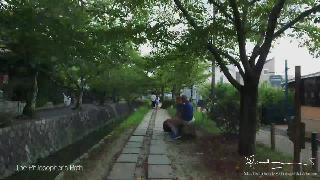
\includegraphics[width=2cm]{img/w2vv_bert/20_target.jpg}};
\node[inner sep=0pt,anchor=west] at (0,0.6)
{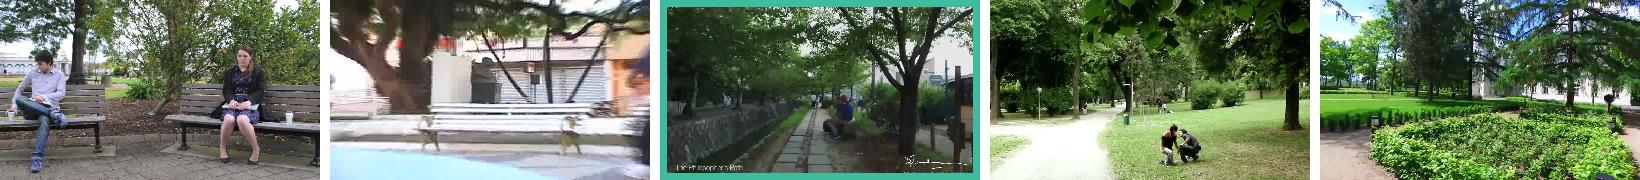
\includegraphics[width=10.25cm]{img/w2vv_bert/20_bert.jpg}};
\node[inner sep=0pt,anchor=west] at (0,-0.6)
{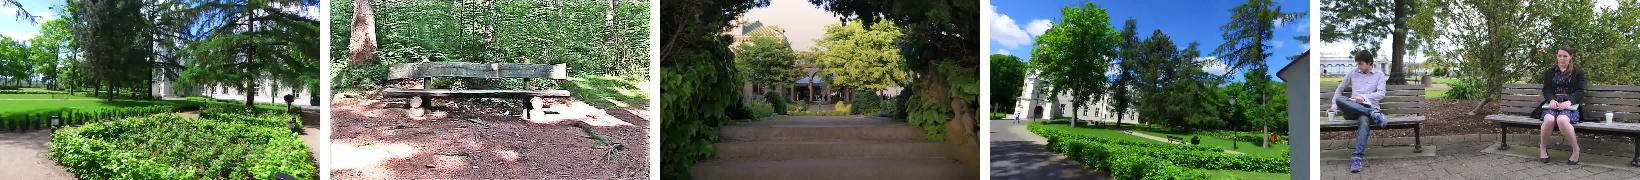
\includegraphics[width=10.25cm]{img/w2vv_bert/20_w2vv.jpg}};
\end{scope}

\begin{scope}[yshift=-3cm]
\node[inner sep=0pt,anchor=west] at (0, 1.4) {\scriptsize A view of a forest in the winter with snow and sunset visible.};
\node[inner sep=0pt,anchor=east] at (-.1, .9) {\scriptsize\texttt{Ours: 1}};
\node[inner sep=0pt,anchor=east] at (-.1, -.9) {\scriptsize\texttt{W2VV: 2}};

\node[inner sep=0pt,anchor=east] at (-.1,0)
{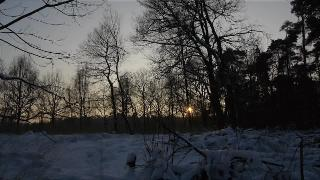
\includegraphics[width=2cm]{img/w2vv_bert/8_target.jpg}};
\node[inner sep=0pt,anchor=west] at (0,0.6)
{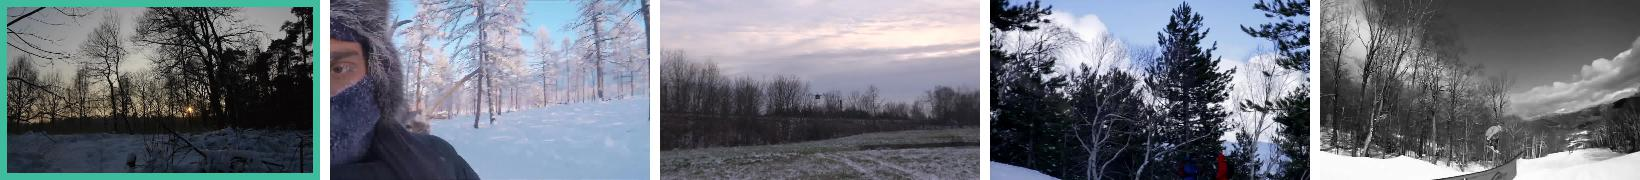
\includegraphics[width=10.25cm]{img/w2vv_bert/8_bert.jpg}};
\node[inner sep=0pt,anchor=west] at (0,-0.6)
{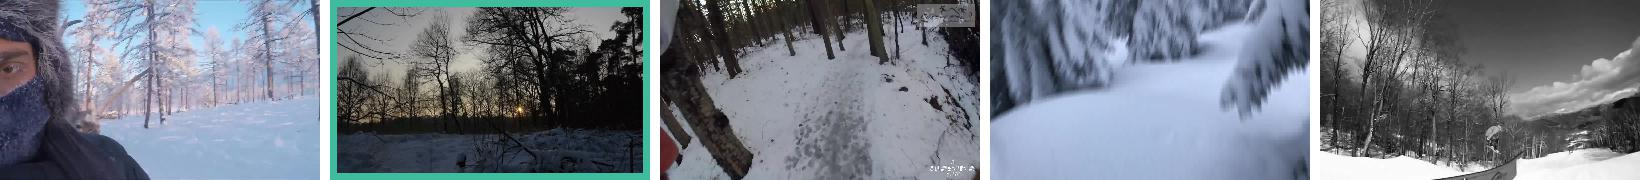
\includegraphics[width=10.25cm]{img/w2vv_bert/8_w2vv.jpg}};
\end{scope}

\begin{scope}[yshift=-6cm]
\node[inner sep=0pt,anchor=west] at (0, 1.4) {\scriptsize A man and woman are depicted in front of coniferous trees.};
\node[inner sep=0pt,anchor=east] at (-.1, .9) {\scriptsize\texttt{Ours: 7}};
\node[inner sep=0pt,anchor=east] at (-.1, -.9) {\scriptsize\texttt{W2VV: 71}};

\node[inner sep=0pt,anchor=east] at (-.1,0)
{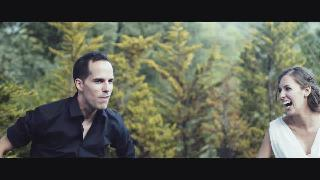
\includegraphics[width=2cm]{img/w2vv_bert/43_target.jpg}};
\node[inner sep=0pt,anchor=west] at (0,0.6)
{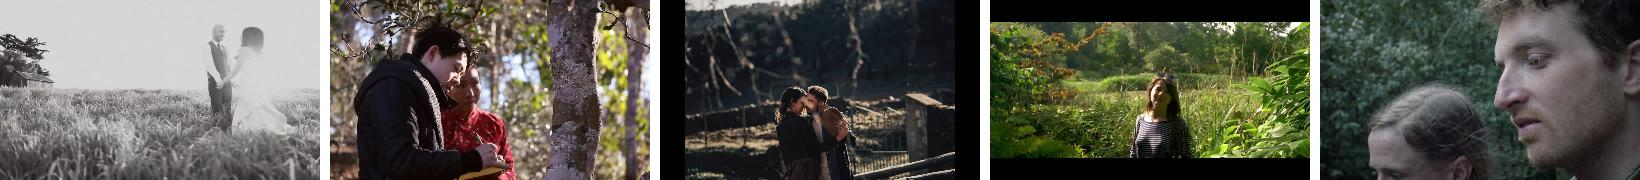
\includegraphics[width=10.25cm]{img/w2vv_bert/43_bert.jpg}};
\node[inner sep=0pt,anchor=west] at (0,-0.6)
{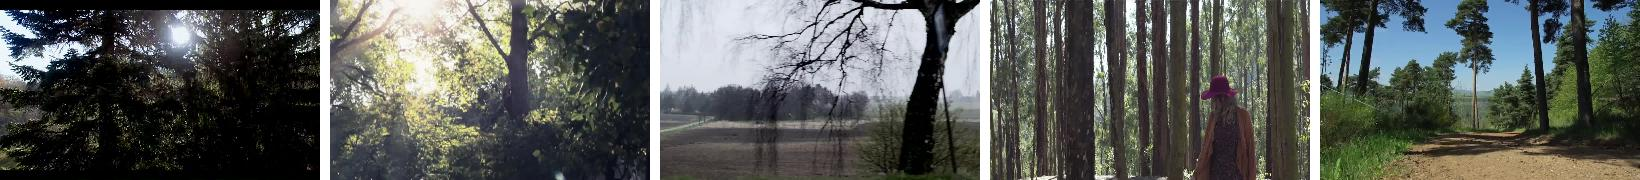
\includegraphics[width=10.25cm]{img/w2vv_bert/43_w2vv.jpg}};
\end{scope}

\begin{scope}[yshift=-9cm]
\node[inner sep=0pt,anchor=west] at (0, 1.4) {\scriptsize A bicycle seat with a bag.};
\node[inner sep=0pt,anchor=east] at (-.1, .9) {\scriptsize\texttt{Ours: 2}};
\node[inner sep=0pt,anchor=east] at (-.1, -.9) {\scriptsize\texttt{W2VV: 116}};

\node[inner sep=0pt,anchor=east] at (-.1,0)
{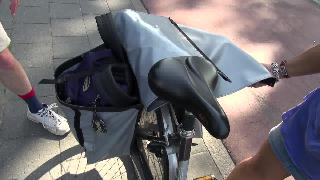
\includegraphics[width=2cm]{img/w2vv_bert/140_target.jpg}};
\node[inner sep=0pt,anchor=west] at (0,0.6)
{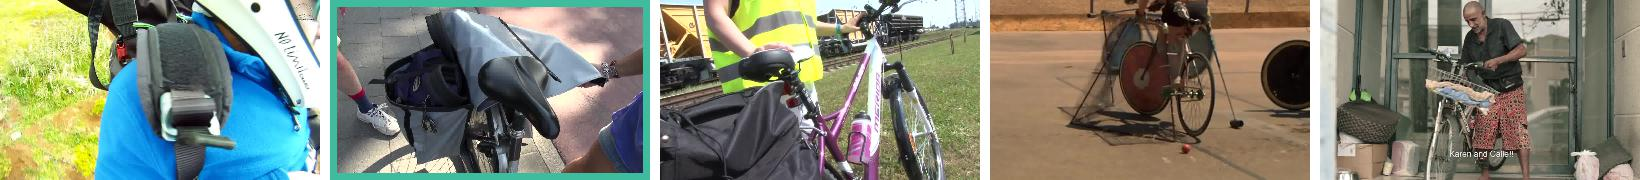
\includegraphics[width=10.25cm]{img/w2vv_bert/140_bert.jpg}};
\node[inner sep=0pt,anchor=west] at (0,-0.6)
{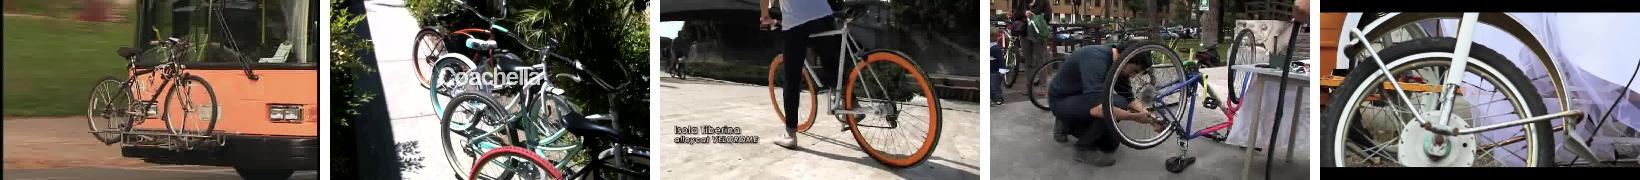
\includegraphics[width=10.25cm]{img/w2vv_bert/140_w2vv.jpg}};
\end{scope}

\begin{scope}[yshift=-12cm]
\node[inner sep=0pt,anchor=west] at (0, 1.4) {\scriptsize A boy sitting at the table and eating breakfast.};
\node[inner sep=0pt,anchor=east] at (-.1, .9) {\scriptsize\texttt{Ours: 2}};
\node[inner sep=0pt,anchor=east] at (-.1, -.9) {\scriptsize\texttt{W2VV: 8}};

\node[inner sep=0pt,anchor=east] at (-.1,0)
{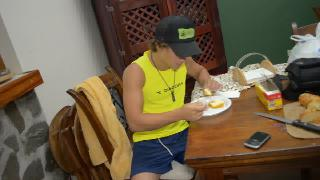
\includegraphics[width=2cm]{img/w2vv_bert/128_target.jpg}};
\node[inner sep=0pt,anchor=west] at (0,0.6)
{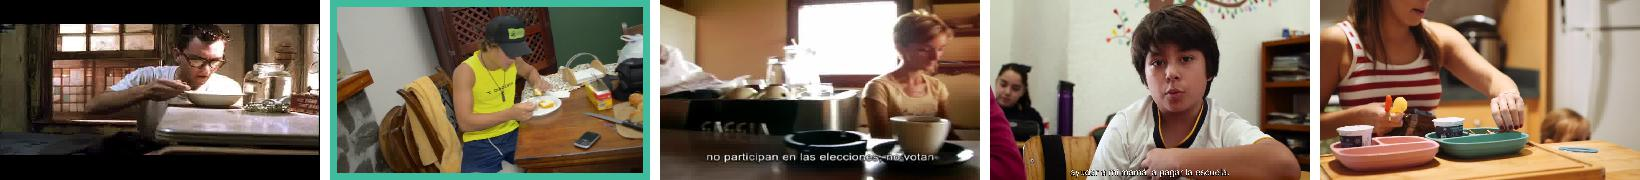
\includegraphics[width=10.25cm]{img/w2vv_bert/128_bert.jpg}};
\node[inner sep=0pt,anchor=west] at (0,-0.6)
{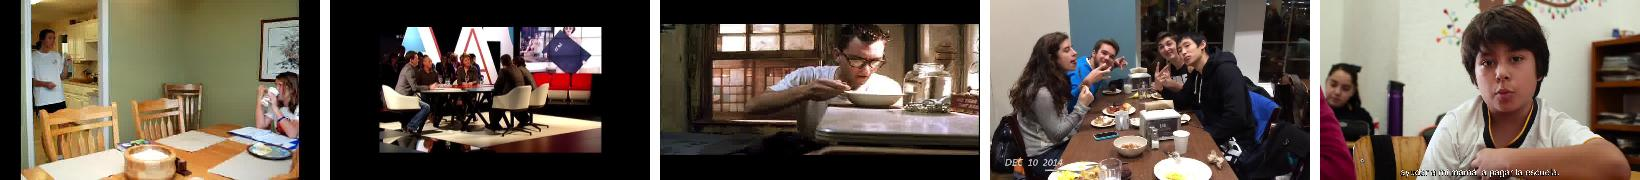
\includegraphics[width=10.25cm]{img/w2vv_bert/128_w2vv.jpg}};
\end{scope}

\begin{scope}[yshift=-15cm]
\node[inner sep=0pt,anchor=west] at (0, 1.4) {\scriptsize Pink and orange gas on the stadium.};
\node[inner sep=0pt,anchor=east] at (-.1, .9) {\scriptsize\texttt{Ours: 18}};
\node[inner sep=0pt,anchor=east] at (-.1, -.9) {\scriptsize\texttt{W2VV: 150}};

\node[inner sep=0pt,anchor=east] at (-.1,0)
{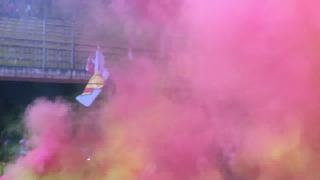
\includegraphics[width=2cm]{img/w2vv_bert/109_target.jpg}};
\node[inner sep=0pt,anchor=west] at (0,0.6)
{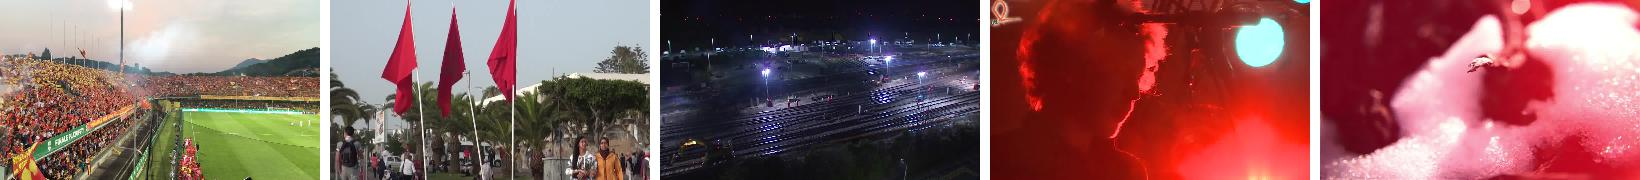
\includegraphics[width=10.25cm]{img/w2vv_bert/109_bert.jpg}};
\node[inner sep=0pt,anchor=west] at (0,-0.6)
{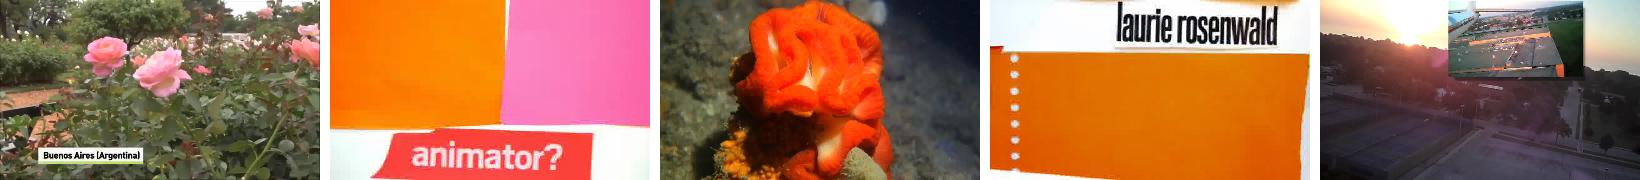
\includegraphics[width=10.25cm]{img/w2vv_bert/109_w2vv.jpg}};
\end{scope}

\end{tikzpicture}
    \caption[Comparison between W2VV++ and our BERT extension, queries in favor of BERT]{Comparison between W2VV++ and our BERT extension on 20k-V3C1 dataset, queries in favor of BERT. Show top 5 results of our model (top) and W2VV++ (bottom) for a given query. The target image is shown on the left with its position according the two models. See Figures \ref{fig:w2vv_bert_comparison_w2vvbetter} and \ref{fig:w2vv_bert_comparison_wrong} for more examples.}
    \label{fig:w2vv_bert_comparison_bertbetter}
\end{figure}

\begin{figure}
    \centering
    \begin{tikzpicture}

\begin{scope}[yshift=0cm]
\node[inner sep=0pt,anchor=west] at (0, 1.4) {\scriptsize An old temple in a desert, blue sky above with a text description.};
\node[inner sep=0pt,anchor=east] at (-.1, .9) {\scriptsize\texttt{Ours: 119}};
\node[inner sep=0pt,anchor=east] at (-.1, -.9) {\scriptsize\texttt{W2VV: 4}};

\node[inner sep=0pt,anchor=east] at (-.1,0)
{
\includegraphics[width=2cm]{img/w2vv_bert/12_target.jpg}};
\node[inner sep=0pt,anchor=west] at (0,0.6)
{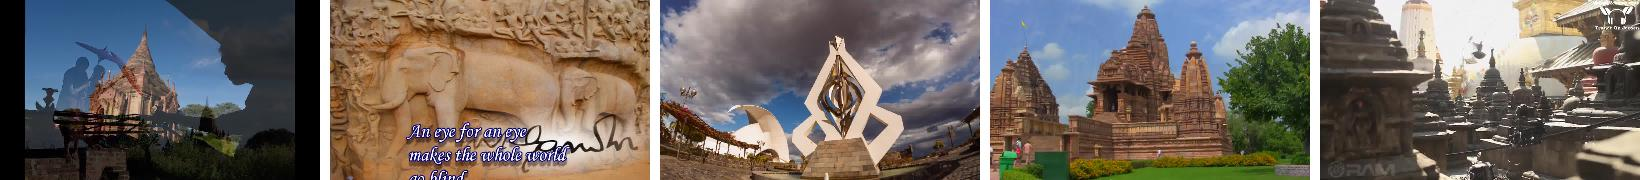
\includegraphics[width=10.25cm]{img/w2vv_bert/12_bert.jpg}};
\node[inner sep=0pt,anchor=west] at (0,-0.6)
{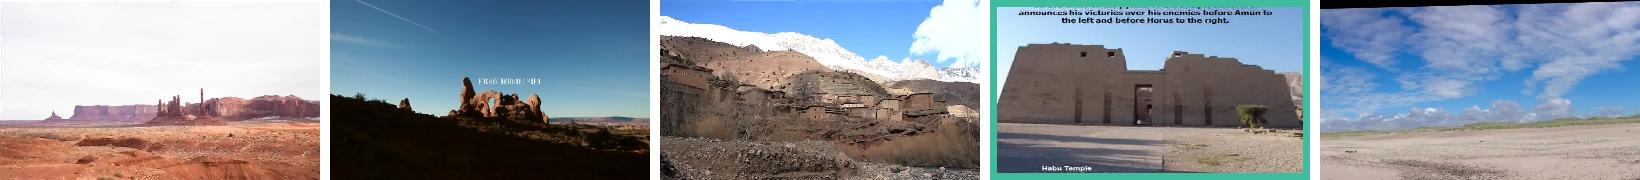
\includegraphics[width=10.25cm]{img/w2vv_bert/12_w2vv.jpg}};
\end{scope}

\begin{scope}[yshift=-3cm]
\node[inner sep=0pt,anchor=west] at (0, 1.4) {\scriptsize Duck on the water surface in the dark.};
\node[inner sep=0pt,anchor=east] at (-.1, .9) {\scriptsize\texttt{Ours: 23}};
\node[inner sep=0pt,anchor=east] at (-.1, -.9) {\scriptsize\texttt{W2VV: 1}};

\node[inner sep=0pt,anchor=east] at (-.1,0)
{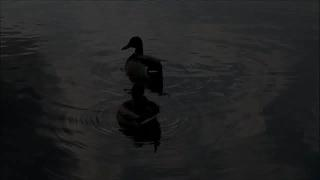
\includegraphics[width=2cm]{img/w2vv_bert/106_target.jpg}};
\node[inner sep=0pt,anchor=west] at (0,0.6)
{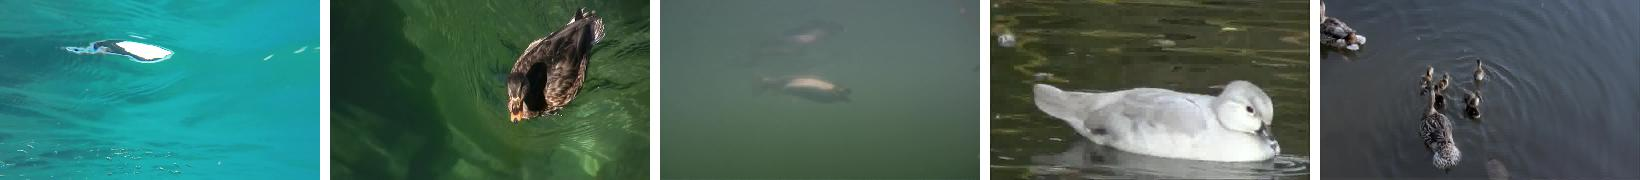
\includegraphics[width=10.25cm]{img/w2vv_bert/106_bert.jpg}};
\node[inner sep=0pt,anchor=west] at (0,-0.6)
{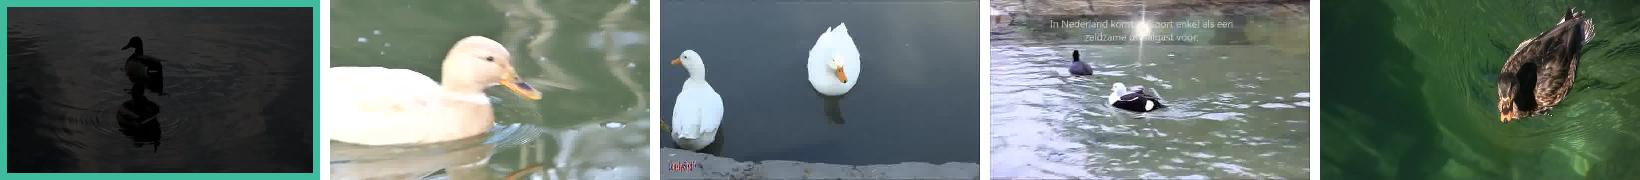
\includegraphics[width=10.25cm]{img/w2vv_bert/106_w2vv.jpg}};
\end{scope}

\begin{scope}[yshift=-6cm]
\node[inner sep=0pt,anchor=west] at (0, 1.4) {\scriptsize A man examining trophy cups on a table, with several books lying around.};
\node[inner sep=0pt,anchor=east] at (-.1, .9) {\scriptsize\texttt{Ours: 38}};
\node[inner sep=0pt,anchor=east] at (-.1, -.9) {\scriptsize\texttt{W2VV: 2}};

\node[inner sep=0pt,anchor=east] at (-.1,0)
{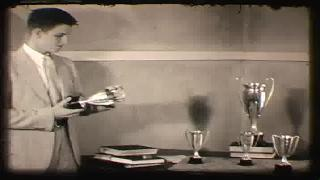
\includegraphics[width=2cm]{img/w2vv_bert/76_target.jpg}};
\node[inner sep=0pt,anchor=west] at (0,0.6)
{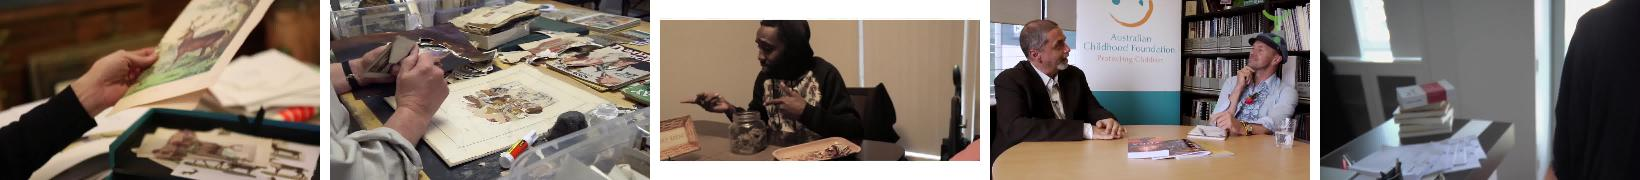
\includegraphics[width=10.25cm]{img/w2vv_bert/76_bert.jpg}};
\node[inner sep=0pt,anchor=west] at (0,-0.6)
{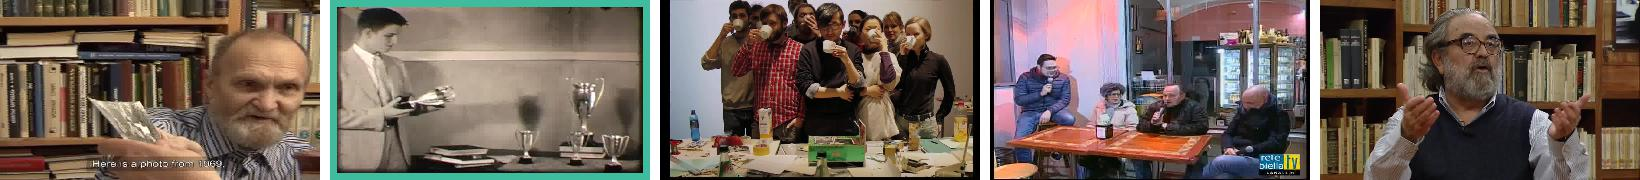
\includegraphics[width=10.25cm]{img/w2vv_bert/76_w2vv.jpg}};
\end{scope}

\begin{scope}[yshift=-9cm]
\node[inner sep=0pt,anchor=west] at (0, 1.4) {\scriptsize A wooden doors which leads to a room with many chairs.};
\node[inner sep=0pt,anchor=east] at (-.1, .9) {\scriptsize\texttt{Ours: 5}};
\node[inner sep=0pt,anchor=east] at (-.1, -.9) {\scriptsize\texttt{W2VV: 1}};

\node[inner sep=0pt,anchor=east] at (-.1,0)
{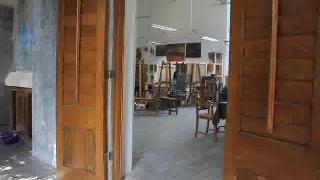
\includegraphics[width=2cm]{img/w2vv_bert/52_target.jpg}};
\node[inner sep=0pt,anchor=west] at (0,0.6)
{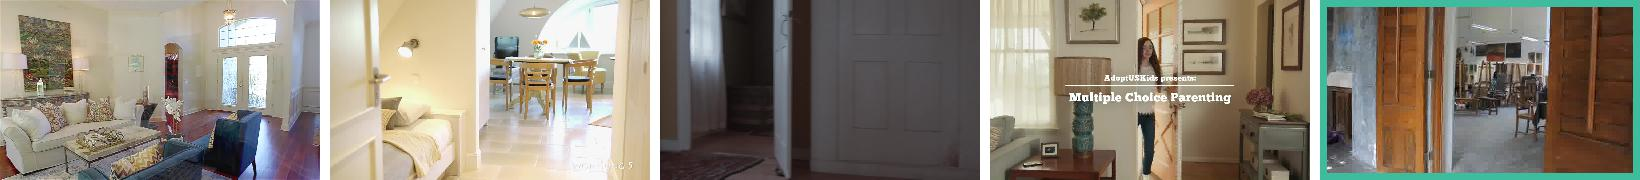
\includegraphics[width=10.25cm]{img/w2vv_bert/52_bert.jpg}};
\node[inner sep=0pt,anchor=west] at (0,-0.6)
{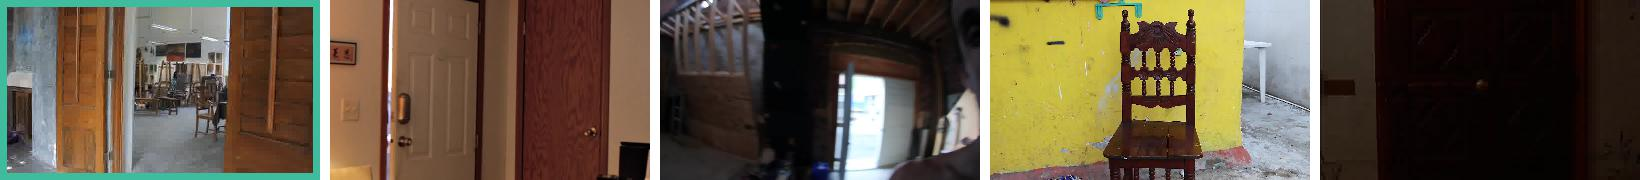
\includegraphics[width=10.25cm]{img/w2vv_bert/52_w2vv.jpg}};
\end{scope}

\end{tikzpicture}
    \caption[Comparison between W2VV++ and our BERT extension, queries in favor of W2VV++]{Continuation of Figure \ref{fig:w2vv_bert_comparison_bertbetter}, queries in favor of W2VV++.}
    \label{fig:w2vv_bert_comparison_w2vvbetter}
\end{figure}

\begin{figure}
    \centering
    \begin{tikzpicture}

\begin{scope}[yshift=0cm]
\node[inner sep=0pt,anchor=west] at (0, 1.4) {\scriptsize A view of a modern house in a city block, with a palm tree in front.};
\node[inner sep=0pt,anchor=east] at (-.1, .9) {\scriptsize\texttt{Ours: 101}};
\node[inner sep=0pt,anchor=east] at (-.1, -.9) {\scriptsize\texttt{W2VV: 21}};

\node[inner sep=0pt,anchor=east] at (-.1,0)
{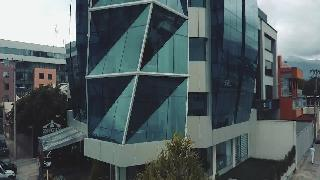
\includegraphics[width=2cm]{img/w2vv_bert/14_target.jpg}};
\node[inner sep=0pt,anchor=west] at (0,0.6)
{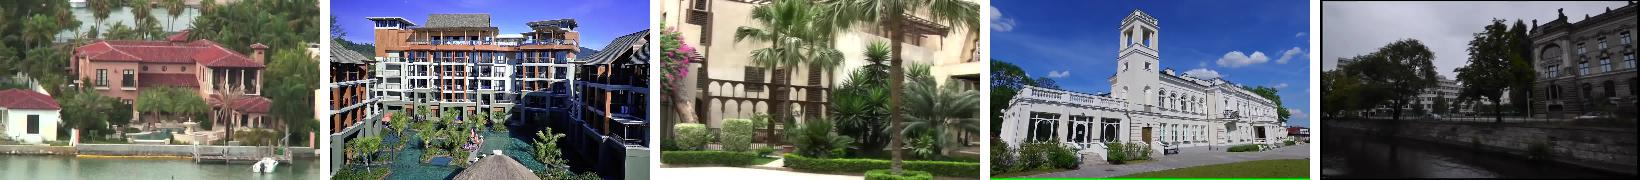
\includegraphics[width=10.25cm]{img/w2vv_bert/14_bert.jpg}};
\node[inner sep=0pt,anchor=west] at (0,-0.6)
{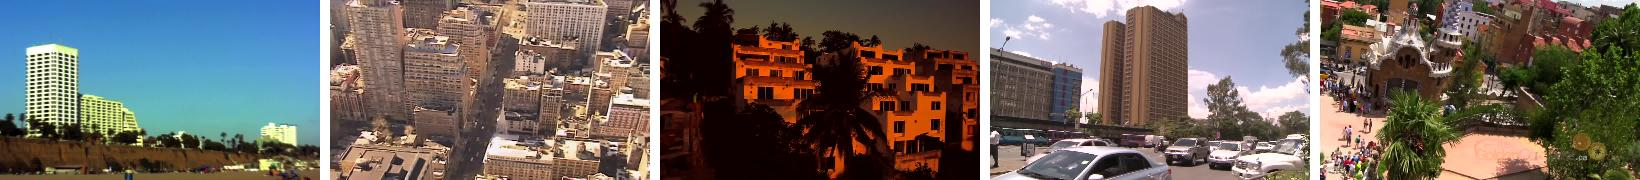
\includegraphics[width=10.25cm]{img/w2vv_bert/14_w2vv.jpg}};
\end{scope}

\begin{scope}[yshift=-3cm]
\node[inner sep=0pt,anchor=west] at (0, 1.4) {\scriptsize On the left a closeup of a woman face, green background on the right.};
\node[inner sep=0pt,anchor=east] at (-.1, .9) {\scriptsize\texttt{Ours: 378}};
\node[inner sep=0pt,anchor=east] at (-.1, -.9) {\scriptsize\texttt{W2VV: 1595}};

\node[inner sep=0pt,anchor=east] at (-.1,0)
{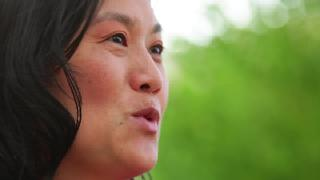
\includegraphics[width=2cm]{img/w2vv_bert/16_target.jpg}};
\node[inner sep=0pt,anchor=west] at (0,0.6)
{
\includegraphics[width=10.25cm]{img/w2vv_bert/16_bert.jpg}};
\node[inner sep=0pt,anchor=west] at (0,-0.6)
{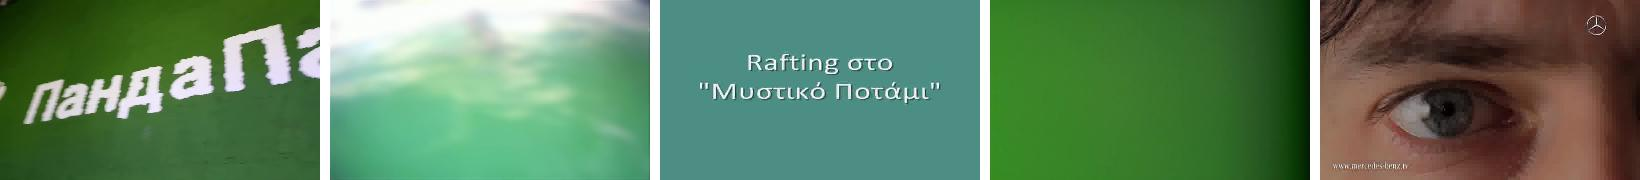
\includegraphics[width=10.25cm]{img/w2vv_bert/16_w2vv.jpg}};
\end{scope}

\begin{scope}[yshift=-6cm]
\node[inner sep=0pt,anchor=west] at (0, 1.4) {\scriptsize Long asphalt road through savanna with bushes and blue sky.};
\node[inner sep=0pt,anchor=east] at (-.1, .9) {\scriptsize\texttt{Ours: 146}};
\node[inner sep=0pt,anchor=east] at (-.1, -.9) {\scriptsize\texttt{W2VV: 5}};

\node[inner sep=0pt,anchor=east] at (-.1,0)
{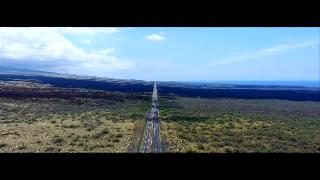
\includegraphics[width=2cm]{img/w2vv_bert/32_target.jpg}};
\node[inner sep=0pt,anchor=west] at (0,0.6)
{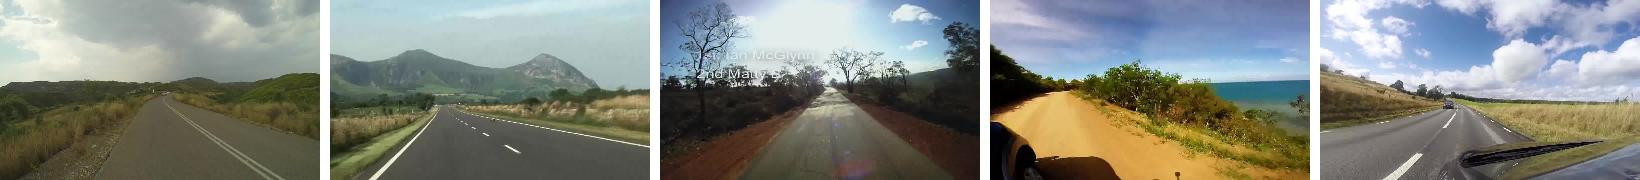
\includegraphics[width=10.25cm]{img/w2vv_bert/32_bert.jpg}};
\node[inner sep=0pt,anchor=west] at (0,-0.6)
{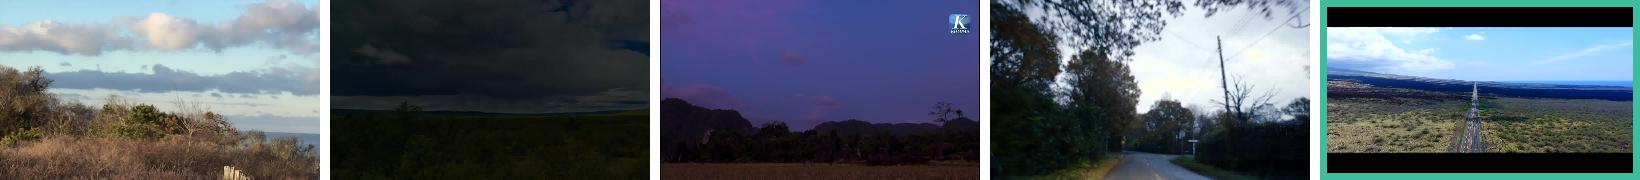
\includegraphics[width=10.25cm]{img/w2vv_bert/32_w2vv.jpg}};
\end{scope}

\end{tikzpicture}
    \caption[Comparison between W2VV++ and our BERT extension, unclear and wrong queries]{Continuation of Figure \ref{fig:w2vv_bert_comparison_bertbetter}, unclear and wrong queries. Even though W2VV++ outperforms our model on the first and third query, its top results do not match the query well.}
    \label{fig:w2vv_bert_comparison_wrong}
\end{figure}



%powerful video embedding
%- pretrained on Soprts1M, Kinetics
%- HowTo100M, weakly supervised

%powerful text embedding
%- bag of words, gru
%- pretrained word2vec
%- transformer based - bert, roberta, xlm-r multilingual

%Datasets:
%MS-COCO \cite{Microsoft COCO: Common objects in context. In: ECCV (2014)} 123 thousand images each with 5 captions
%Flickr30K \cite{From image descriptions to visual denotations: New similarity metrics for semantic inference over event descriptions. In: ACL (2014)} containing 31,000+ (over 30 thousand) images collected from Flickr website with five captions each.
%Tumblr GIF (TGIF) \cite{https://arxiv.org/pdf/1604.02748.pdf}, with 100K animated GIFs from Tumblr and 120K natural language descriptions obtained
%MSR-VTT \cite{MSR-VTT: A Large Video Description Dataset for Bridging Video and Language} dataset contains 10K web video clips and 200k natural sentences describing the visual content of the clips
%The MSVD dataset contains 1970 Youtube clips, and each video is annotated with around 40 sentences.

%utilizing multilingual bert adds queries in other languages for free:)
%going back to "concept-based" approach
%- using only BoW 'kind of' makes the model concept-based.